\documentclass{article}
\usepackage[utf8]{inputenc}
\usepackage{graphicx}
\usepackage{polski}
\usepackage{verbatim}
\usepackage{subfig}
\usepackage{geometry}
\usepackage{listings}
\usepackage{hyperref}

\date{}
\begin{document}
	\begin{figure}[h]
		\centering
		\Huge{Symulacja rozprzestrzeniania się dymu}
		\vspace{15mm}
		
		
\includegraphics[scale = 0.23]{eaiib.jpg}
		
\includegraphics[scale = 0.5]{agh.jpg}
		
\includegraphics[scale = 0.65]{IT.jpg}
		
		\vspace{15mm}
		
		\centering
		\large Opiekun projektu:
		
		\Large dr inż. Robert Lubaś
	\end{figure}
	
	\vspace{25mm}
	\begin{center}
		\Large{Marcin Sawczuk \hspace{5mm} Daniel Warloch \hspace{5mm} Norbert Pilarek }
	\end{center}
	\vspace{12mm}
	\begin{center}
		\large{Informatyka II rok \\ Wydział Elektrotechniki, Automatyki,
			Informatyki i Inżynierii Biomedycznej \\
			Akademia Górniczo-Hutnicza im. Stanisława Staszica
			w Krakowie} 
		
		\medskip
		\Large{2019/2020}
	\end{center}
	
	\pagebreak
	\tableofcontents
	\pagebreak
	
	\section{Wstęp}
	Przepływ powietrza wokół samochodu. Fala po uderzeniu meteorytu. Cyrkulacja krwi w układzie krążenia. Wszystkie te zjawiska łączy obecność płynów: cieczy i gazów. W niniejszej pracy próbujemy poznać naukę poświęconą symulowaniu wyżej wspomnianych i wielu innych zjawisk: obliczeniową mechanikę płynów (CFD – Computational Fluid Dynamics).
	
	\medskip
	\medskip
	\noindent Głównym zadaniem projektu było stworzenie trójwymiarowego modelu rozprzestrzeniania się dymu w pomieszczeniu. Model uwzględnia m.in. takie czynniki jak temperatura czy kierunek ruchu powietrza. W tej pracy opracowaliśmy model oraz przedstawiliśmy wyniki symulacji 3D dymu.
	
	\medskip
	\medskip
	\noindent Nasza symulacja mimo początkowo innych koncepcji ostatecznie opiera się na Równaniach Naviera-Stokesa. Są to równania różniczkowe cząstkowe drugiego rzędu. Operują na polach prędkości i~ciśnień, badając ich ewolucję w czasie. Równania Naviera-Stokesa stanowią bardzo dojrzały, dokładnie zgłębiony dział mechaniki płynów.
	
	\vspace{12mm}
	\section{Teoria}
	\vspace{3mm}
	\subsection{Równania Naviera-Stokesa}
	Równania Naviera-Stokesa pozwalają zamodelować szeroki wachlarz zjawisk fizycznych. Aby uprościć zagadnienie potraktujmy powietrze jako nieściśliwy płyn niutonowski. Nieściśliwość płynu oznacza, iż jego gęstość pozostaje stała w całej przestrzeni, co jest słusznym przybliżeniem przy niewielkich prędkościach przepływu.
	
	\medskip
	\medskip
	\noindent Wyprowadzenie równań Naviera-Stokesa wykracza poza materiał tego sprawozdania; znacznie bardziej wyczerpujące opracowanie tematu można znaleźć m.in. w [7]. Równania Naviera-Stokesa dla nieściśliwego płynu niutonowskiego mają następującą postać:
	$$
	\frac{\partial \mathbf{u}}{\partial t} =-(\mathbf{u} \cdot \nabla) \mathbf{u}-\frac{1}{d} \nabla p+\nu \nabla^{2} \mathbf{u}+\mathbf{f} 
	$$
	$$
	\nabla \cdot \mathbf{u} =0
	$$
	gdzie u – prędkość płynu, d – gęstość płynu, p – ciśnienie, $\nu$ – lepkość kinematyczna, f – wypadkowa sił zewnętrznych działających na płyn.
	
	\medskip
	\medskip
	\noindent Pierwsze równanie jest przekształconą drugą zasadą dynamiki Newtona dla płynów i stanowi równanie pędu. Człony tego równania można opisać następująco:
	\begin{itemize}
		\item \( \frac{\partial \mathbf{u}}{\partial t} \quad \) pochodna prędkości po czasie
		
		\item \( -(\mathbf{u} \cdot \nabla) \mathbf{u} \quad \) człon adwekcyjny (konwekcyjny). Jest odpowiedzialny za przemieszczanie się prędkości płynu w przestrzeni z upływem czasu.
		
		\item \( -\frac{1}{d} \nabla p \quad \) człon ciśnieniowy. Reprezentuje siły występujące wewnątrz płynu na skutek różnicy ciśnień miedzy różnymi obszarami płynu.
		
		\item \( \nu \nabla^{2} \mathbf{u} \quad \) Człon lepkościowy. Reprezentuje występujące wewnątrz płynu siły tarcia, zachodzące między obszarami o różnych prędkościach. Znaczenie tych sił determinuje lepkość kinematyczna płynu, oznaczona przez \( \nu . \)
		
		\item f \( \quad \) Siły zewnętrzne. Wypadkowa sił działających na płyn, ale nie mających źródła w samym płynie.
	\end{itemize}
	
	\medskip
	\medskip
	\noindent Równanie drugie stanowi warunek nieściśliwości – wymusza, by ilość płynu wpływającego do danego obszaru przestrzeni była równa ilości płynu wypływającego.
	
	\vspace{7mm}
	\subsection{Ważne pojęcia}
	\vspace{3mm}
	\renewcommand*\thesubsubsection{}
	\subsubsection{Układ dyspersyjny} 
	Układ, zwykle koloidalny, złożony z co najmniej dwóch faz, z których przynajmniej jedną stanowi silnie rozdrobniony materiał, rozproszony w drugiej fazie o charakterze ciągłym, zwanej ośrodkiem dyspersyjnym. Obie fazy mogą być dowolne, muszą się jednak różnić między sobą składem lub stanem skupienia.
	
	\vspace{4mm}
	\subsubsection{Dym} 
	Układem dyspersyjny (koloidalnym) , w którym fazą ciągłą (rozpraszającą) jest powietrze, a fazą rozproszoną są cząsteczki substancji; Układy dyspersyjne możemy podzielić wg stanu skupienia faz, dymy zaliczą się do aerozoli; dymy tworzące się w atmosferze z przedostających się do niej stałych produktów np. spalania paliw (z kotłowni, pojazdów) lub pochodzących z innej działalności przemysłowej (jak cementownie), zawierające m.in. cząstki sadzy, popiołu, niespalonego paliwa (aerozole atmosferyczne), powodują skażenie środowiska; dym wytwarza się też celowo, np. w walce zbrojnej (zasłona dymna).
	
	\vspace{4mm}
	\subsubsection{Symulacje CFD dymu}    
	Polegają na komputerowym odtworzeniu danego budynku lub pomieszczenia, a następnie wywołaniu w nim cyfrowego pożaru. Modele 3D pokazują szereg istotnych parametrów, jak na przykład prędkość rozprzestrzeniania dymu, temperaturę oraz efektywność systemów oddymiania. W ten sposób można odwzorować nawet najbardziej niekorzystne scenariusze pożaru. Jest to niezwykle szybka i skuteczna metoda na zweryfikowanie warunków ewakuacji oraz warunków w jakich swoje działania prowadzić będzie jednostka ratowniczo-gaśnicza.
	
	\vspace{12mm}
	\section{Realizacja}
	\subsection{Założenia projektowe}
	\vspace{3mm}
	
	\subsubsection{Narzędzie}
	Staraliśmy się nie używać najczęściej wybieranych programów do przedstawiania symulacji dymu oraz pobierania z tego danych i łatwego ich przedstawienia. Po przejrzeniu dostępnych opracowań zauważyliśmy, że najczęściej stosowanym narzędziem jest Pyrosim. Mimo widocznych zalet postanowiliśmy przebadać inne dostępne możliwości. W dalszej części przedstawimy drogę jaką przeszliśmy, aż do momentu gdy natrafiliśmy na narzędzie które jednocześnie sprostało naszym wymaganiom oraz nie posiadało zbyt wysokiego progu wejścia.
	
	
	\subsubsection{Miejsce}
	Chcieliśmy wykonać projekt, który dotyczy również i nas samych. Miejscem które jest jednym z~najczęściej odwiedzanych przez całą naszą trójkę jest nasza uczelnia. Zrozumieliśmy już na samym początku, że nie posiadamy i nie będziemy posiadać sprzętu, który w rozsądnym czasie dokona nam potrzebnych obliczeń, aby to mógł być ogromny pożar powodujący zadymienie na tak wielkim obszarze jakim jest nasz kampus AGH. Zabraliśmy się za budynek, w którym najprawdopodobniej najczęściej jesteśmy będąc na uczelni, a chodzi o C2. Nasze trudności spowodowały konieczność kolejnych zmian, o których napisaliśmy dalej.
	
	
	\subsubsection{Wizualizacja}
	Zależało nam na tym, aby przedstawione wyniki przemawiały jak najlepiej do nas, wszyscy jak się okazało jesteśmy wzrokowcami. Podążając za tym postawiliśmy na opieranie się w swoim projekcie na danych przedstawionych w przestrzeni 3D. Skupiliśmy się na trzech parametrach, które według nas w tym aspekcie są najważniejsze:
	\begin{itemize}
		\item widoczność - do jej przedstawienia użyliśmy widoku roznoszenia się cząstek
		\item temperatura - zastosowaliśmy wizualizację kolorystyczną, gdzie jaśniejszy kolor oznacza wyższą temperaturę
		\item gęstość - zastosowaliśmy wizualizację kolorystyczną, gdzie jaśniejszy kolor oznacza większą gęstość
	\end{itemize}
	
	\vspace{7mm} 
	\subsection{Ewolucja pomysłu wykonania}
	
	\medskip
	\medskip
	\subsubsection{Python}
	Pierwszym pomysłem na realizację symulacji był język Python w wersji 3. Jest to język wysokiego poziomu. Jego największą zaletą jest prostota składni, ogromna dostępność różnego typu bibliotek oraz pakietów do wizualizacji oraz przeprowadzania symulacji. Ponadto jest to żywy język, a więc jest ciągle rozwijany. 
	
	\medskip
	\vspace{4mm}
	\subsubsection{Pyjet}
	\noindent Po przejrzeniu dostępnych bibliotek wybraliśmy bibliotekę pyjet. Jednak niepowodzenie w zainstalowania jej po wielogodzinnych próbach zmusiła nas do porzucenia tego pomysłu.
	
	\medskip
	\vspace{4mm}
	\subsubsection{Fluidity}
	\noindent Kolejnym naszym odkryciem było dependency o nazwie fluidity, które miało nas wesprzeć w zainstalowaniu wcześniej wspomnianej biblioteki oraz bibliotek z rodziny numpy. Niestety zainstalowanie go zajęło kilkanaście godzin, gdyż wymagane było wiele dodatkowych aplikacji i bibliotek wymaganych do kompilacji naszego celu. Jednak nie poddaliśmy się i po kilku dniach osiągnęliśmy sukces. 
	
	\medskip
	\vspace{4mm}
	\subsubsection{Wyświetlanie}
	\noindent Po uruchomieniu kilku przykładów podanych w dokumentacji postanowiliśmy stworzyć coś własnoręcznie. Jednak bardzo słaby kunszt wykonania dokumentacji tej biblioteki oraz brak możliwości wyświetlania wyników sumulacji w modelu 3D skłoniło nas  do zatrzymania się i zastanowienia się co robić dalej.
	
	\medskip
	\vspace{4mm}
	\subsubsection{Konsultacje}
	\noindent Po zastanowieniu się postanowiliśmy skonsultować z prowadzącym w celu uzyskania profesjonalnej porady. Przedstawiliśmy mu przebytą przez nas drogę. Doradził nam abyśmy wrócili do wyboru oprogramowania które wykorzystamy do wykonania projeku i jeszcze raz dokonali przeglądu dostępnych na rynku rozwiązań. 
	
	
	\medskip
	\vspace{4mm}
	\subsubsection{Blender}
	\noindent Aby rozwiązać ten problem zamiast realizować symulację i pobierać z niej tablicę wyników, a potem obrazować wyniki na płaszczyźnie 3D, postanowiliśmy realizować ją od razu na modelu 3D. W tym celu zastosowaliśmy framework napisany w naszej bibliotece pyjet w Blenderze. Jednak ponownie bardzo słaba dokumentacja zmusiła nas do rezygnacji z tego pomysłu.
	
	\medskip
	\vspace{4mm}
	\subsubsection{MantaFlow}
	\noindent Po ponownym rozejrzeniu się wśród dostępnych rozwiązań i uwzględnieniu naszych poprzednich komplikacji i wyciągniętych wniosków, z pomocą przyszedł nam framework MantaFlow dostępny w~programie Blender od wersji 2.82. 
	
	\vspace{10mm}
	\subsection{Ostateczna technologia}
	\vspace{2mm}
	\textbf{Blender} – wolne i otwarte oprogramowanie do modelowania i renderowania obrazów oraz animacji trójwymiarowych
	
	\medskip
	\medskip
	\noindent \textbf{MantaFlow} w Blenderze jest open-source framework'iem symulującym zachowanie płynów w grafice komputerowym i uczeniu maszynowym. Większość jest zaimplementowana w C++, jednak ustawianie parametrów płynu poprzez skrypty jest zaimplementowane w pythonie, a same posługiwanie się w niej jest bardzo intuicyjne i przyjemne. 
	
	\medskip
	\medskip
	\noindent Do interpretacji wyników symulacji wykorzystujemy \textbf{MantaFlowGUI}`, która także jest bardzo pomocna i łatwa w obsłudze.
	
	
	\vspace{10mm}
	\subsection{Implementacja}
	\vspace{2mm}
	W programie Blender stworzyliśmy rozwiązanie pozwalające na automatyzację procesu tworzenia symulacji dymu z wykorzystaniem MantaFlow a także skryptów w języku Python. Owe rozwiązanie wykorzystuje 3 kolekcje obiektów w programie Blender do wygenerowania źródła dymu, domeny i~effectorów. Natomiast w 4-tej kolekcji umieszczamy kamery z których chcemy uzyskać obraz. 
	
	\vspace{7mm}
	\begin{figure}[h]
		\centering
		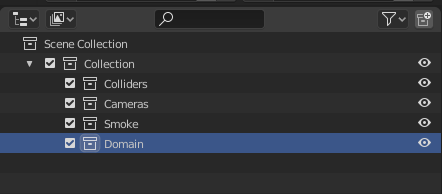
\includegraphics[scale = 1.0]{s1.png}
		\caption{Kolekcje obiektów w programie Blender.}
	\end{figure}
	\vspace{7mm}
	
	\noindent Pierwszym przykładem, który chcieliśmy stworzyć był model całego budynku C2, jednak koszt obliczeniowy przeprowadzenia symulacji rozchodzenia się cząsteczek w tej skali był zbyt duży. Ostatecznie naszym punktem startowym i miejscem do którego się ograniczamy jest sala 429. 
	
	\begin{figure}
		\centering
		\includegraphics[scale = 0.1]{C2.png}
		\caption{Model budynku C2 w Blenderze.}
		
		\vspace{12mm}
		\includegraphics[scale = 0.1]{429.png}
		\caption{Model sali 429 w Blenderze.}
	\end{figure}
	
	\pagebreak
	\medskip
	\vspace{12mm}
	\noindent Aby nasza symulacja była uniwersalna oraz łatwa w obsłudze do ustawiania parametrów dymu, efektorów i domeny stosujemy skrypty napisane w Pythonie.
	\vspace{7mm}
	
	\medskip
	\begin{figure}[ht!]
		\centering
		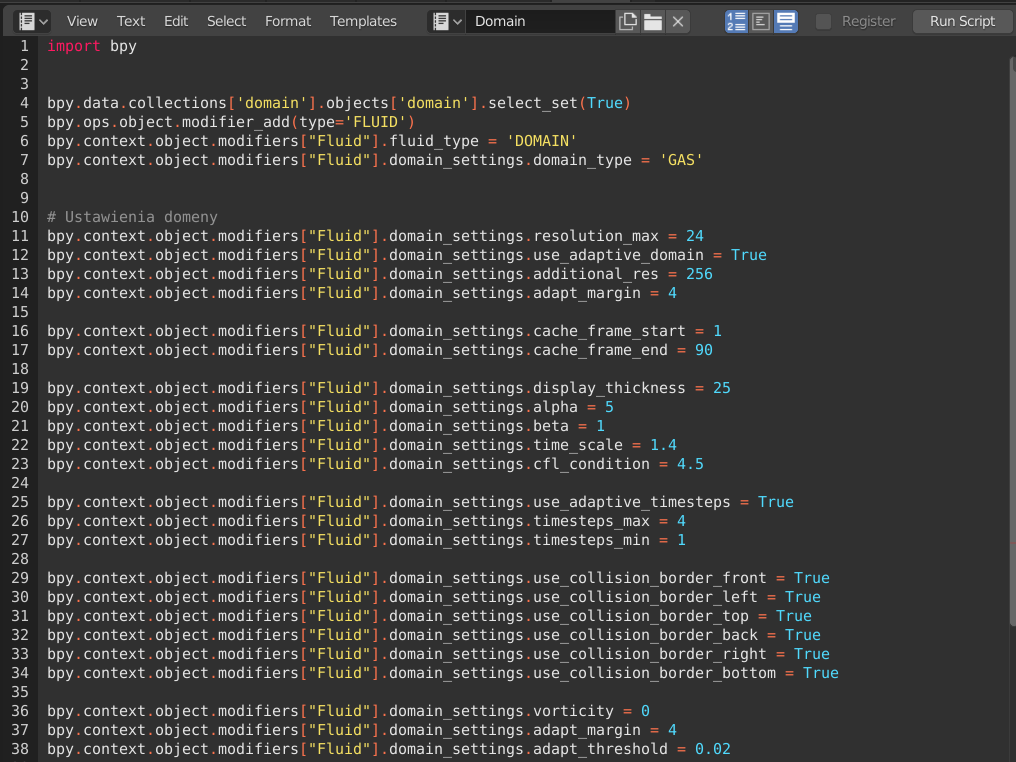
\includegraphics[scale = 0.6]{sk2.png}
		\caption{Przykładowy fragment skryptu napisanego w Pythonie odpowiedzialny za ustawienie parametrów dymu.}
	\end{figure}
	
	\vspace{15mm}
	\medskip
	\noindent Dodatkowo stworzyliśmy wizualizację kolorystyczną m.in. temperatury i gęstości dymu.
	
	\vspace{4mm}
	\begin{figure}[ht!]
		\centering
		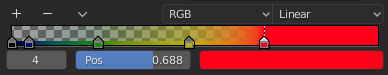
\includegraphics[scale = 1.0]{wizualizacja.png}
		\caption{Utworzona wizualizacja kolorystyczna.}
	\end{figure}
	
	\medskip
	\noindent Aby mieć możliwość pomiaru temperatury, gęstości i innych parametrów dymu w danym punkcie przestrzeni napisaliśmy skrypt pozwalający zwizualizować otrzymane wyniki stosując aplikację MantaFlowGUI, która po zaznaczeniu danego fragmentu dymu dostarcza wszystkich interesujących nas informacji.
	
	\vspace{7mm}
	\begin{figure}[ht!]
		\centering
		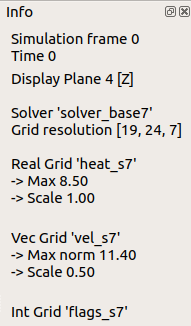
\includegraphics[scale = 0.7]{gui_1.png}
		\caption{Przykładowy fragment wyświetlanych danych w MantaFlowGui.}
	\end{figure}
	
	\vspace{9mm}
	\begin{figure}[ht!]
		\centering
		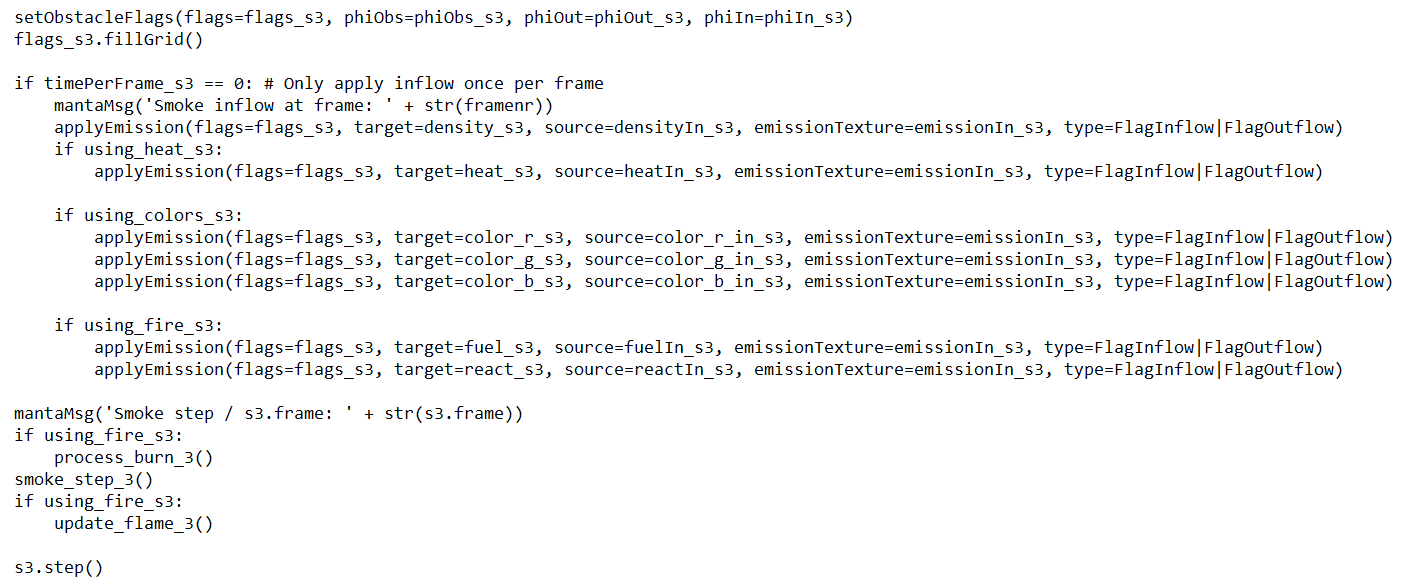
\includegraphics[scale = 0.5]{skrypt_GUI.png}
		\caption{Przykładowy fragment skryptu odpowiedzialnego za wyświetlanie parametrów \\ w MantaFlowGui.}
	\end{figure}
	
	
	\pagebreak
	\subsection{Symulacje}
	Jak już wcześniej wspomnieliśmy, nasza przykładowa symulacja ma miejsce w sali 429. 
	
	\vspace{4mm}
	\subsubsection{Pierwsza symulacja}
	Na biurku wybucha pożar, z którego dym rozprzestrzenia się po całym pomieszczeniu.
	
	\vspace{7mm}
	\begin{figure}[ht!]
		\centering
		\includegraphics[scale = 0.08]{s1_1.png}
		\caption{Pierwsza symulacja.}
	\end{figure}
	
	\vspace{7mm}
	\begin{figure}[ht!]
		\centering
		\includegraphics[scale = 0.08]{s1_2.png}
		\caption{Pierwsza symulacja.}
	\end{figure}
	
	\newpage
	W 230 klatce następuje "ugaszenie pożaru", otworzenie wszystkich okien oraz włączenie systemu oddymiania.
	
	\vspace{7mm}
	\begin{figure}[ht!]
		\centering
		\includegraphics[scale = 0.08]{s1_3.png}
		\caption{Pierwsza symulacja.}
	\end{figure}
	
	\vspace{2mm}
	\subsubsection{Druga symulacja}
	W tym wariancie temperatura emitera jest 4 razy większa niż w poprzednim punkcie, a reszta założeń jest taka sama.
	
	\vspace{7mm}
	\begin{figure}[ht!]
		\centering
		\includegraphics[scale = 0.08]{s2_1.png}
		\caption{Druga symulacja.}
	\end{figure}
	
	\newpage
	\subsubsection{Trzecia symulacja}
	\medskip
	W tym modelu występują 2 źródła dymu, jedno na biurku, jak w wcześniejszych wariantach, a~drugie na przeciwległym końcu sali. Źródło znajdujące się na biurku ma 16 razy większą temperaturę emitera, a reszta założeń jest identyczna z wcześniejszymi punktami.
	
	\vspace{25mm}
	\begin{figure}[ht!]
		\centering
		\includegraphics[scale = 0.11]{s3_2.png}
		\caption{Trzecia symulacja.}
	\end{figure}
	
	\vspace{7mm}
	\begin{figure}[ht!]
		\centering
		\includegraphics[scale = 0.1]{s3_1.png}
		\caption{Trzecia symulacja.}
		
		\vspace{15mm}
		\centering
		\includegraphics[scale = 0.1]{s3_3.png}
		\caption{Trzecia symulacja.}
	\end{figure}
	
	
	\newpage
	\subsection{Wyniki}
	
	\vspace{7mm}
	\begin{figure}[ht!]
		\centering
		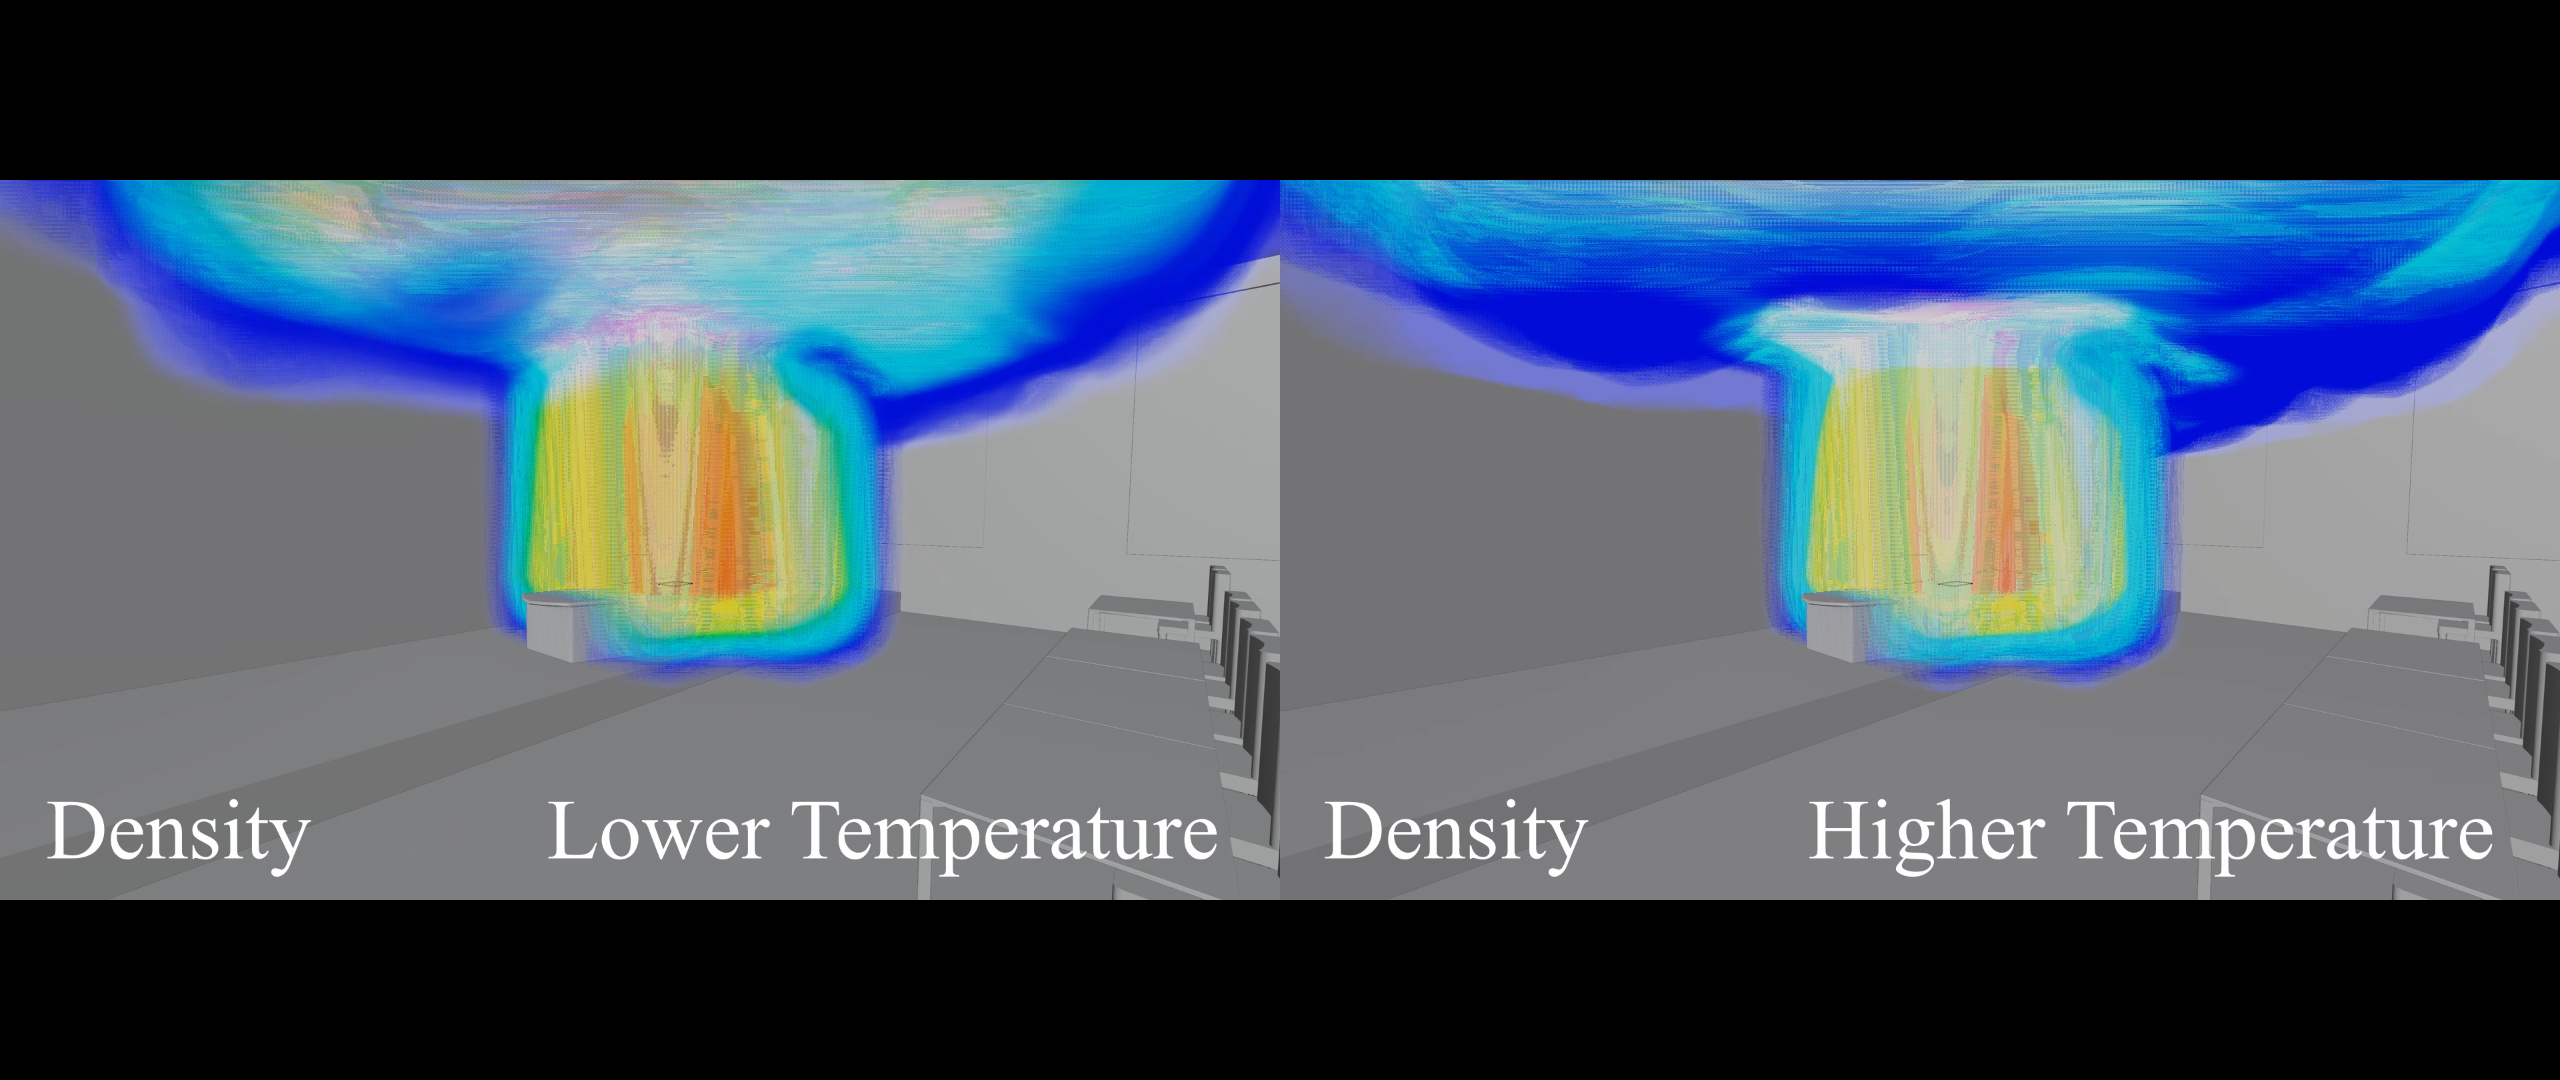
\includegraphics[scale = 0.15]{1.png}
		\caption{Porównanie gęstości dymu przy różnych temperaturach źródła zadymienia.}
	\end{figure}
	
	\vspace{15mm}
	\begin{figure}[ht!]
		\centering
		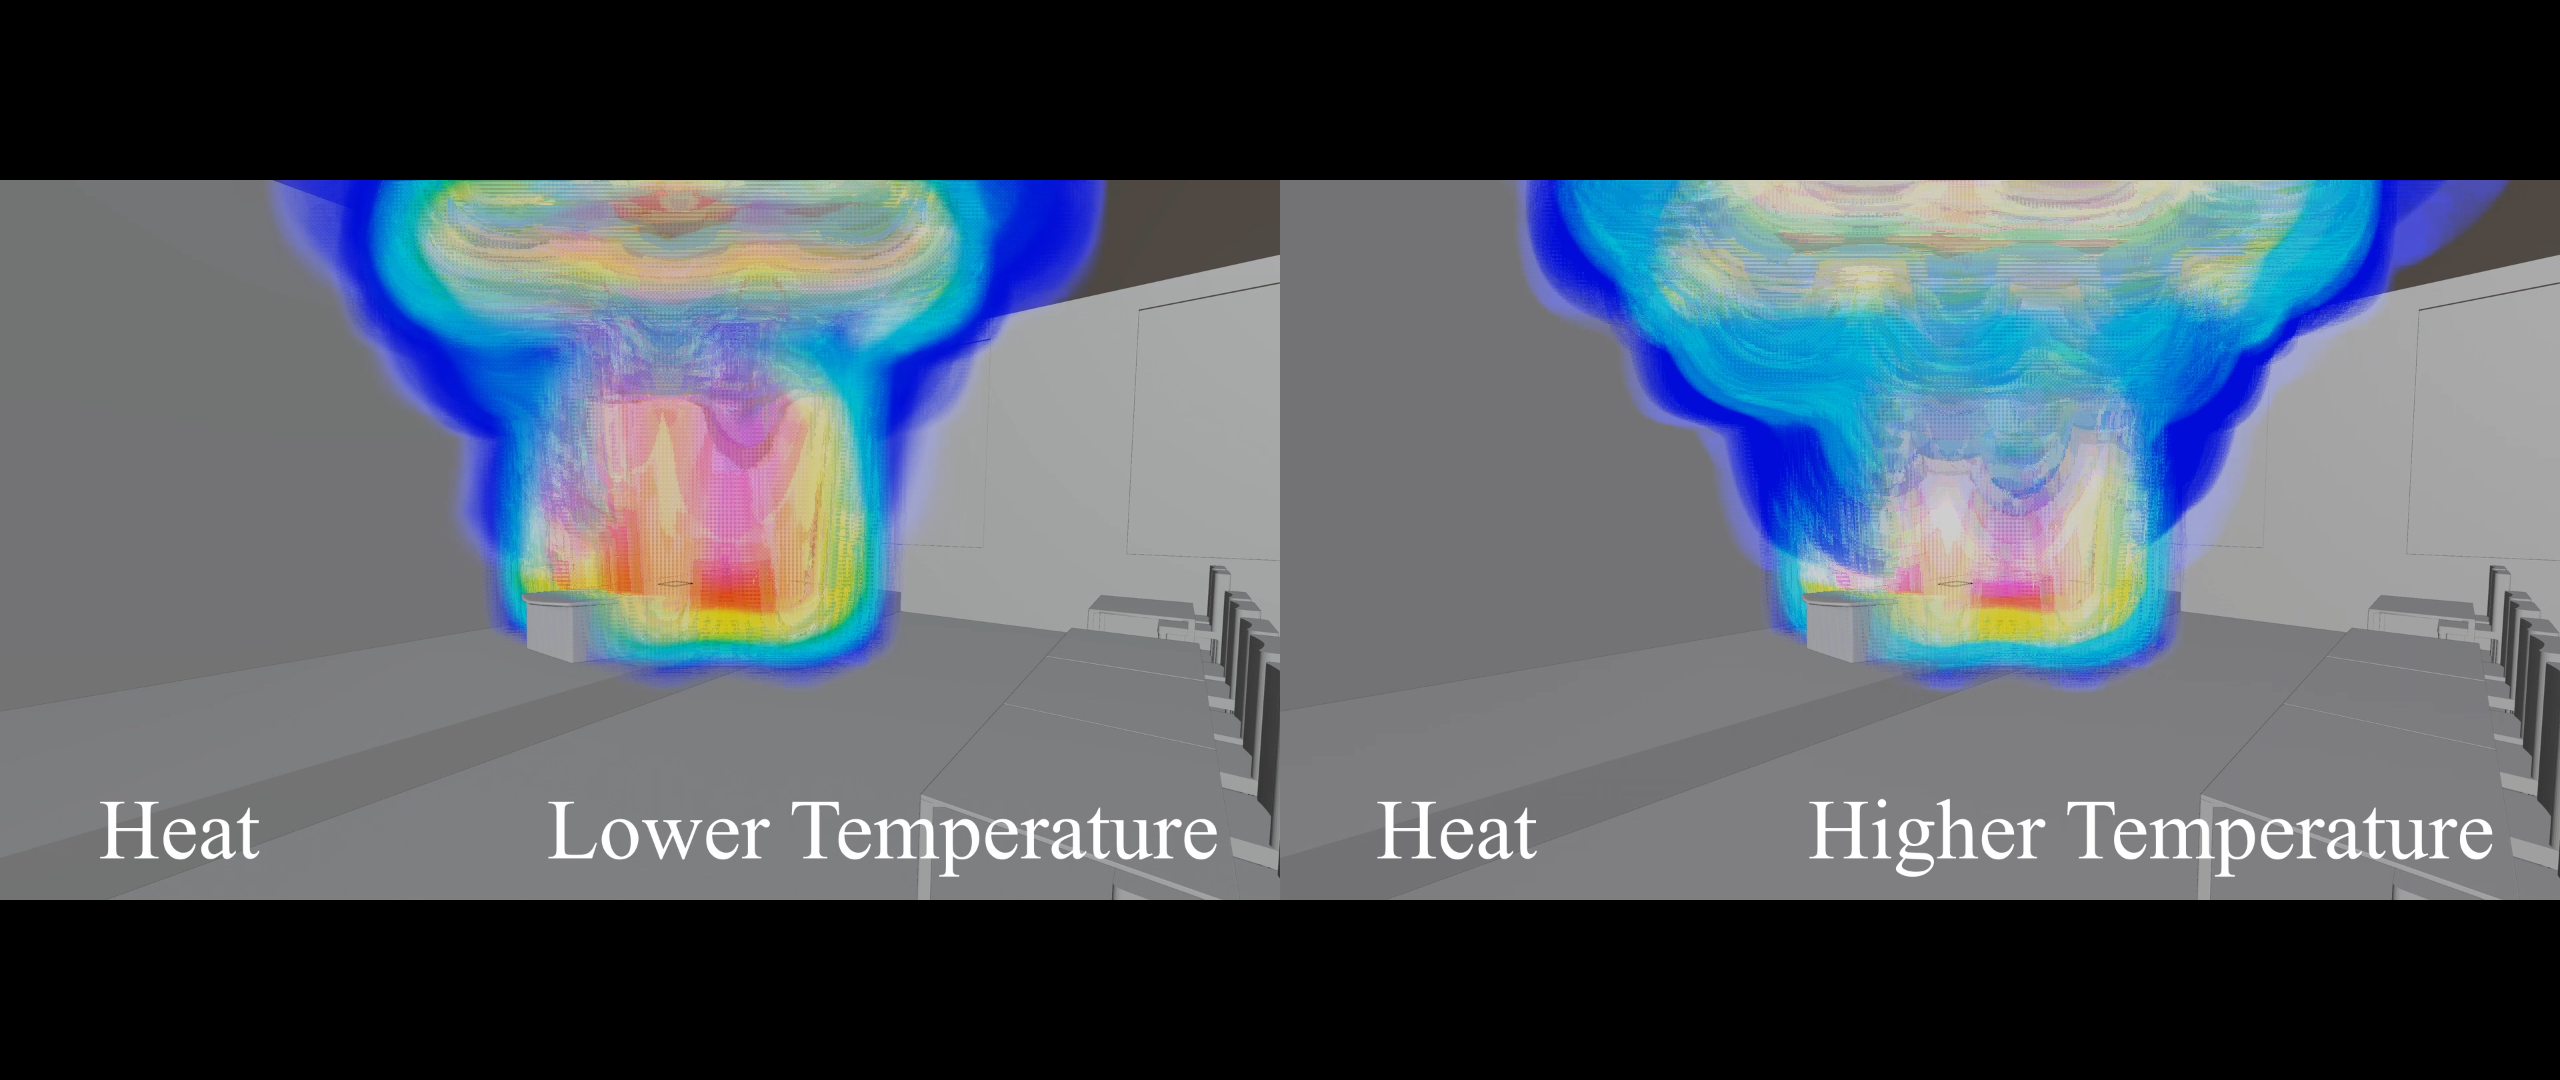
\includegraphics[scale = 0.15]{2.png}
		\caption{Porównanie ciepła dymu przy różnych temperaturach źródła zadymienia.}
	\end{figure}
	
	\begin{figure}[ht!]
		\centering
		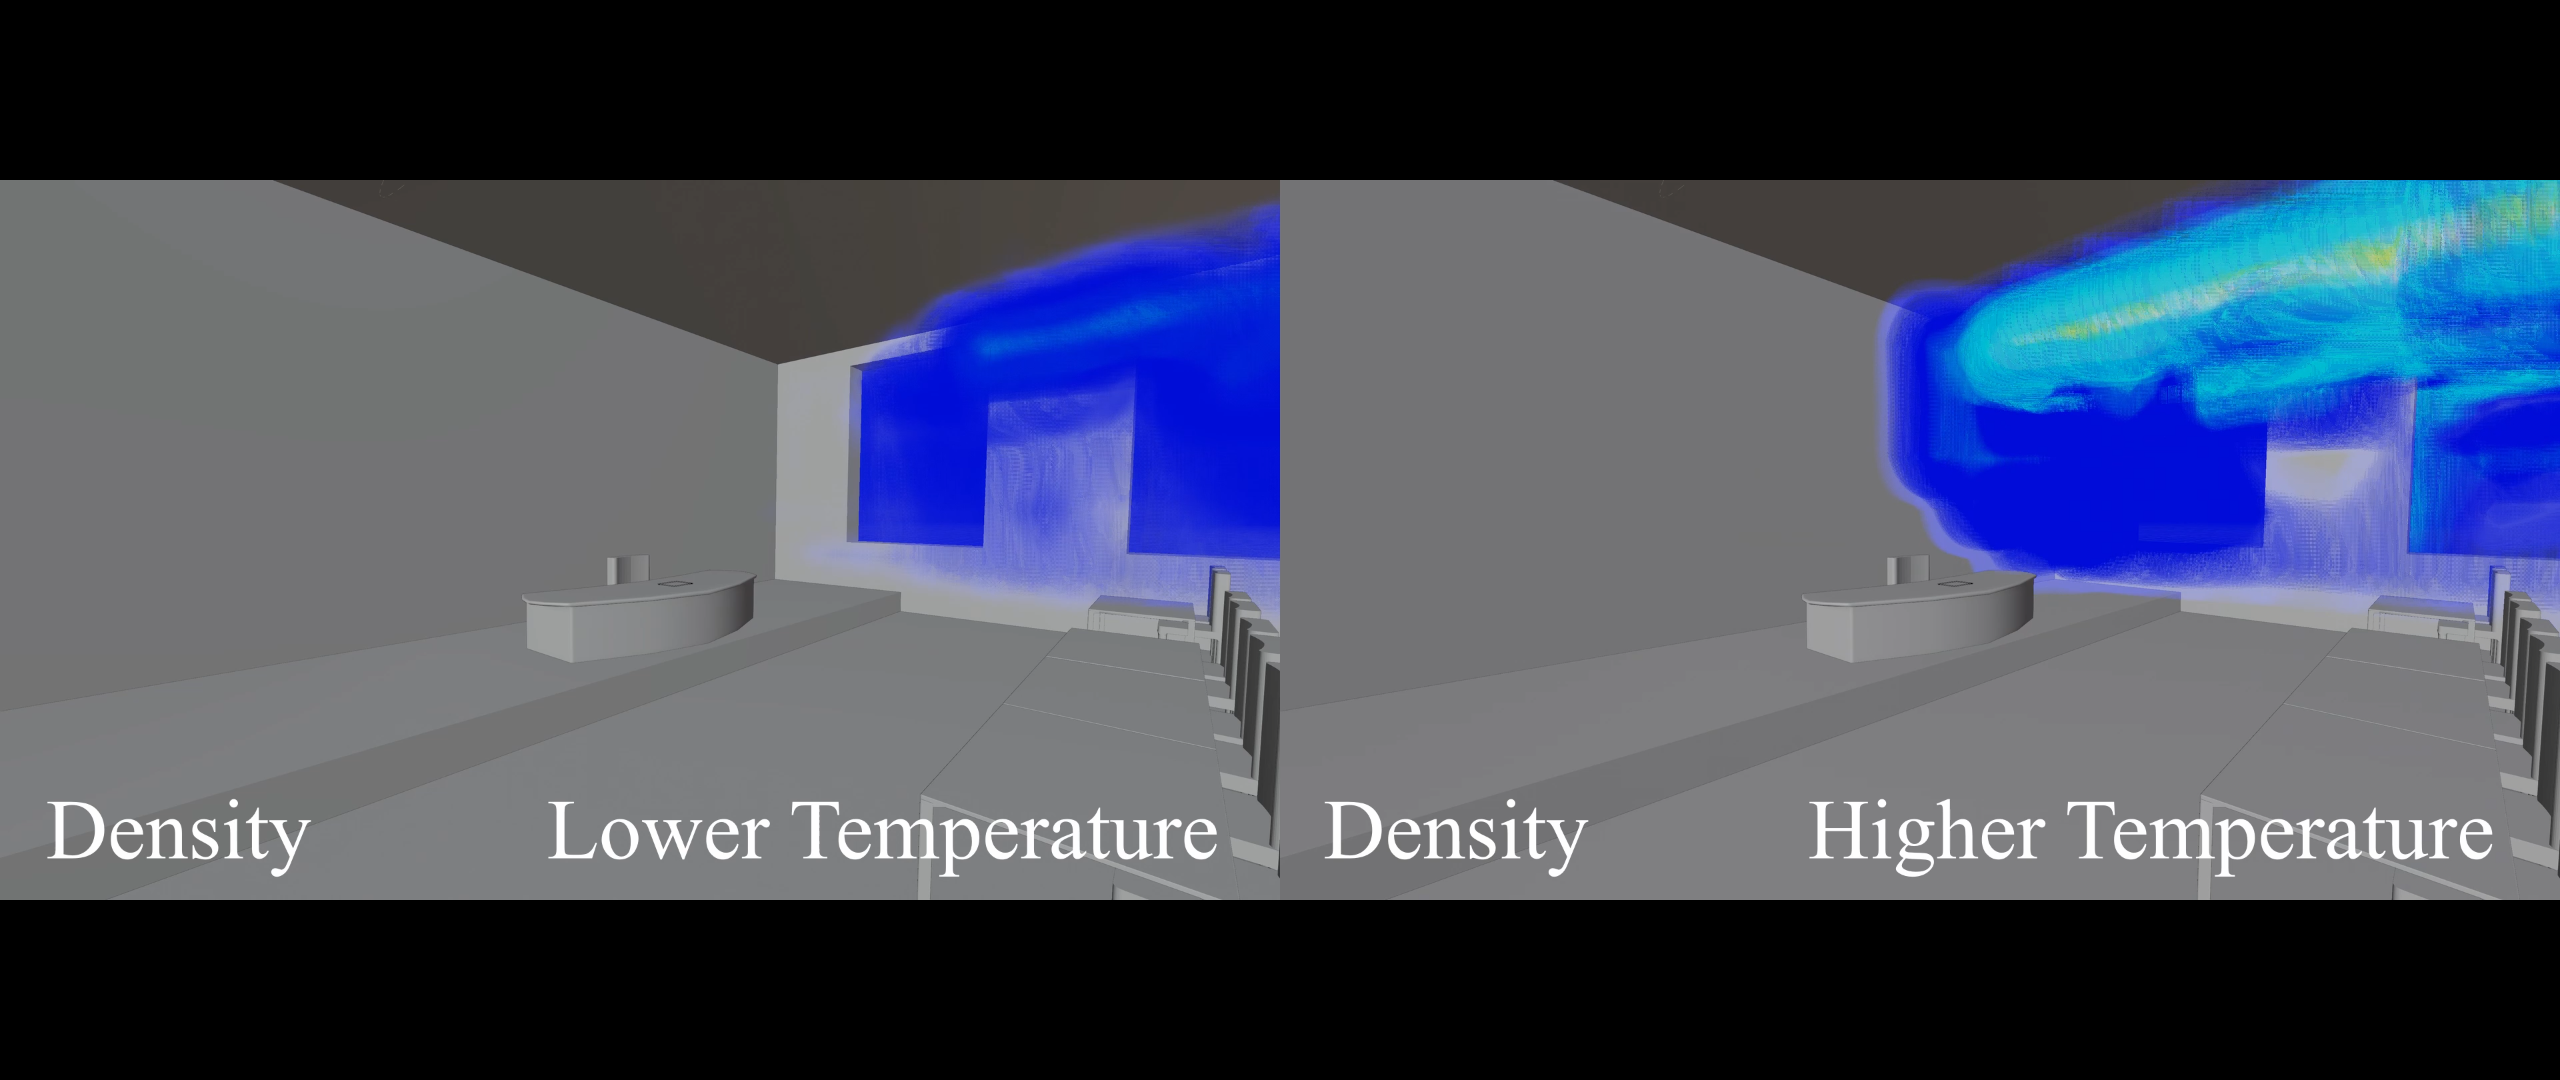
\includegraphics[scale = 0.165]{3.png}
		\caption{Porównanie gęstości dymu przy różnych temperaturach źródła zadymienia.}
		
		\vspace{45mm}
		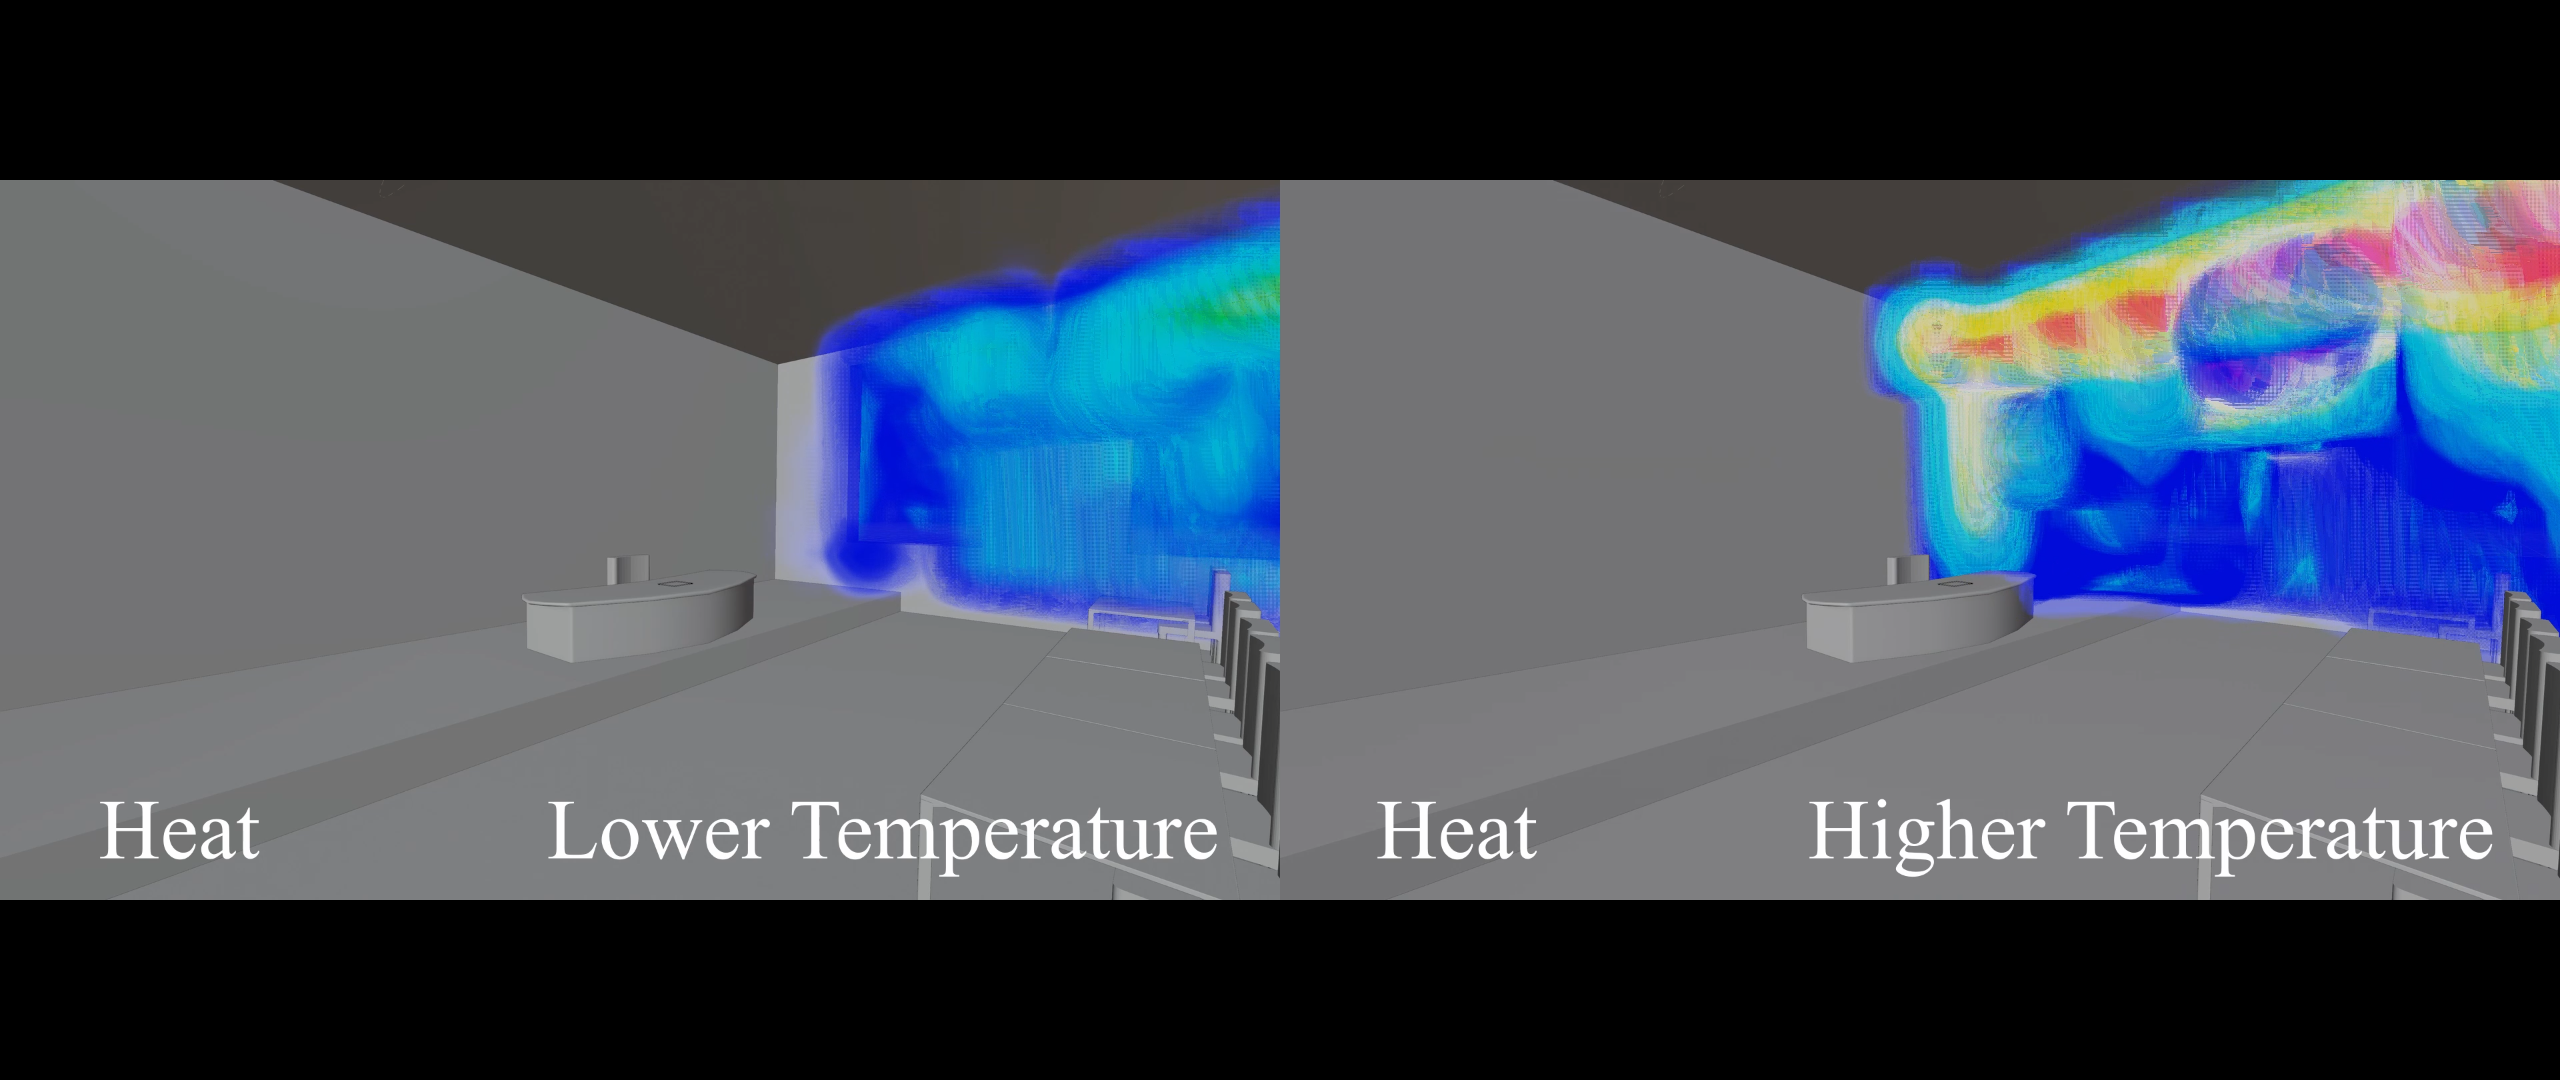
\includegraphics[scale = 0.165]{4.png}
		\caption{Porównanie ciepła dymu przy różnych temperaturach źródła zadymienia.}
	\end{figure}
	
	\pagebreak
	
	\begin{figure}[ht!]
		\centering
		\includegraphics[scale = 0.111]{starcie.png}
		\caption{Starcie się dymów o różnych temperaturach źródła zadymienia.}
	\end{figure}
	
	\pagebreak
	
	\begin{figure}[ht!]
		\centering
		\medskip
		\medskip
		\medskip
		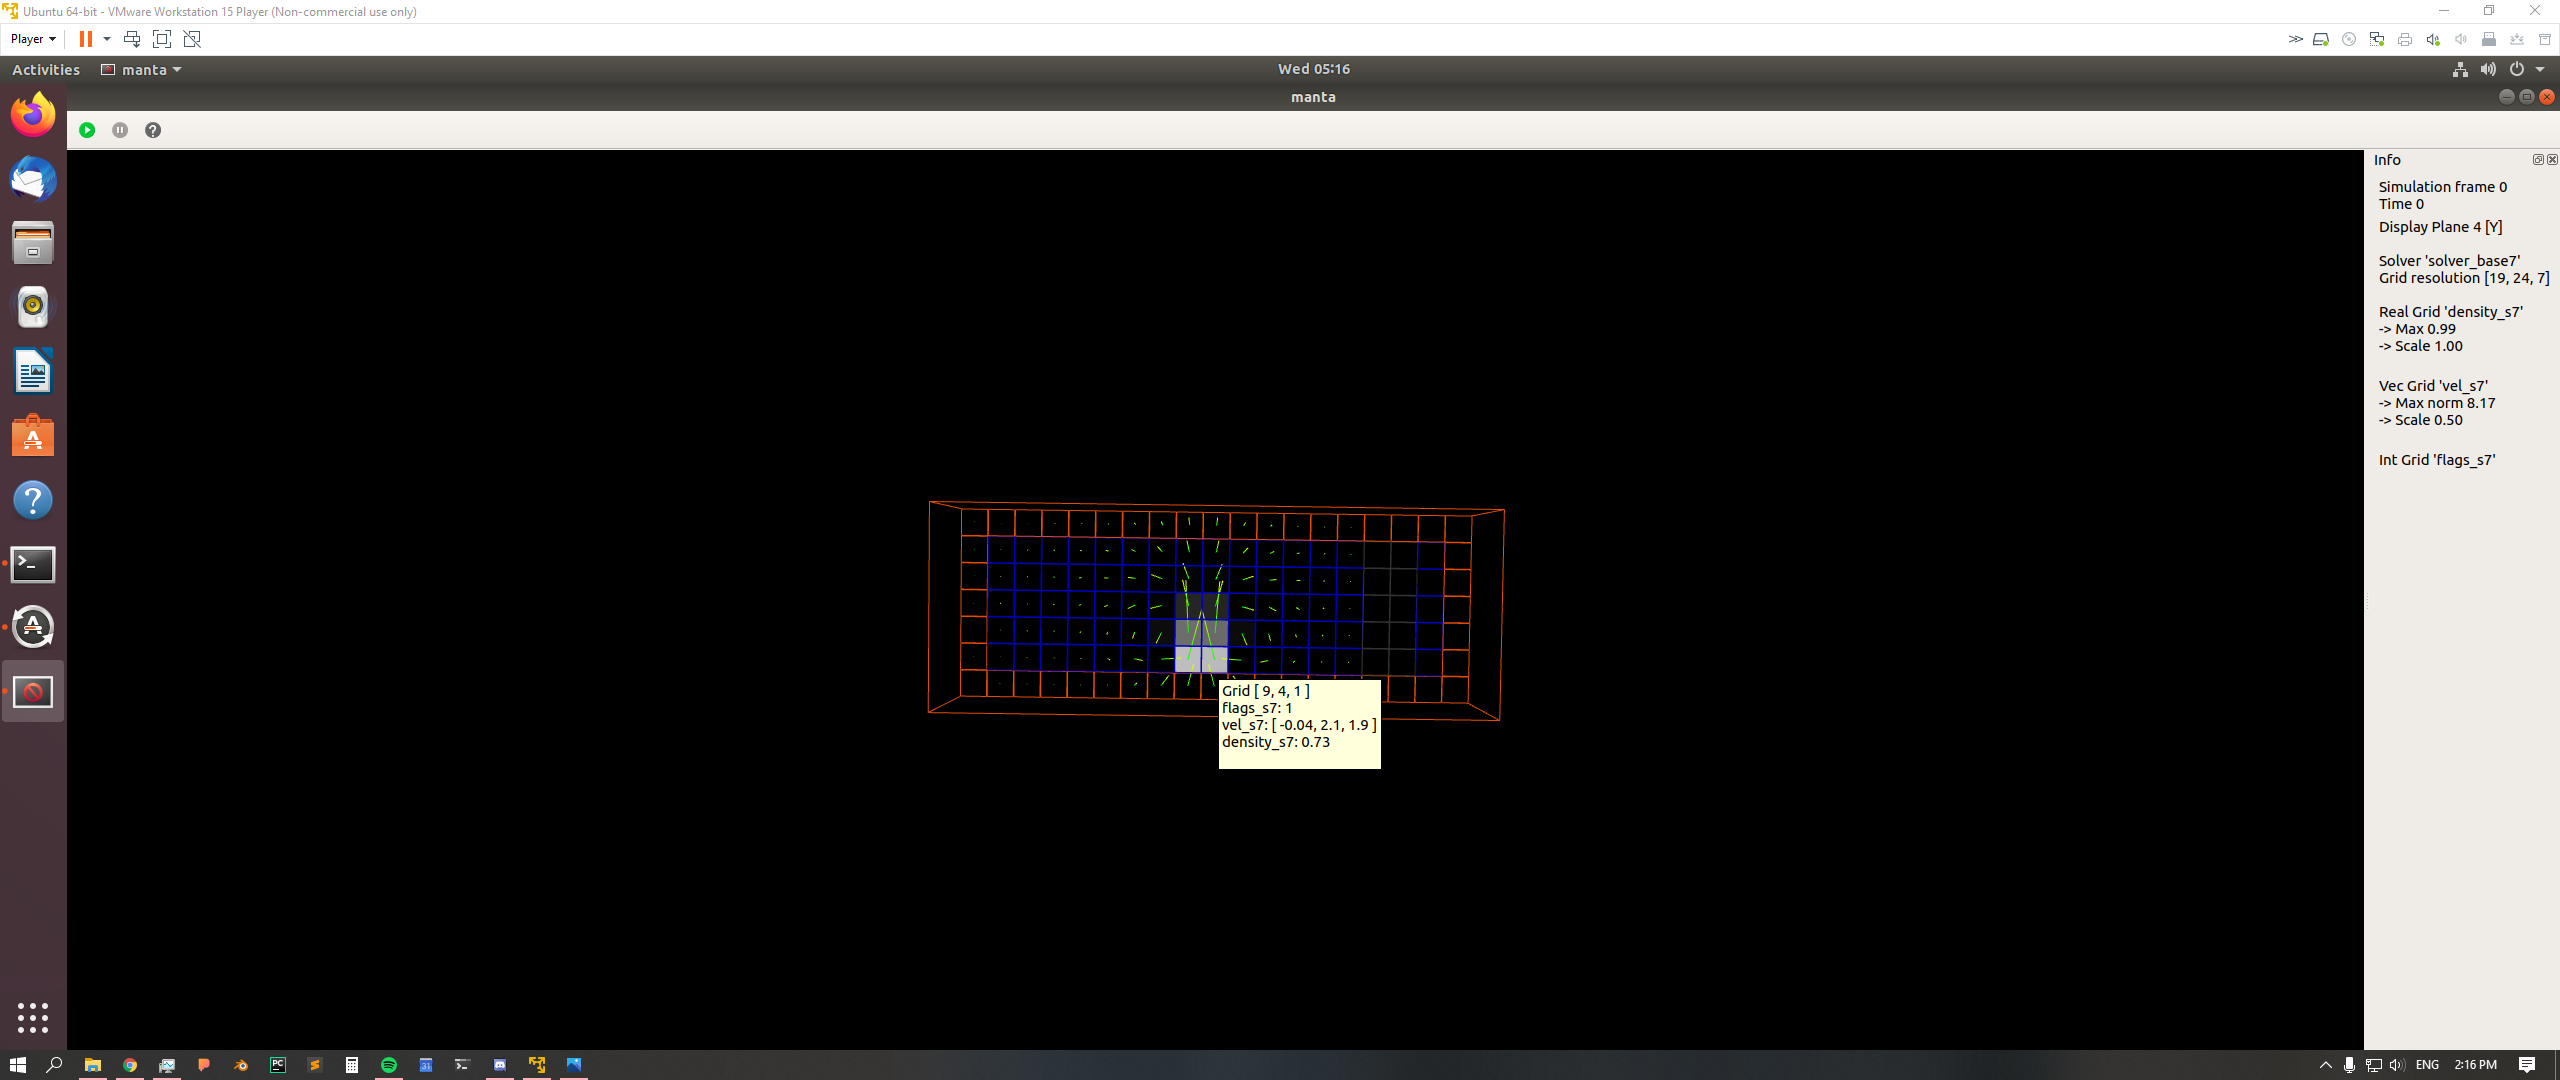
\includegraphics[scale = 0.165]{mgui_1.png}
		\caption{Gęstość dymu.}
	\end{figure}
	
	\vspace{15mm}
	\begin{figure}[ht!]
		\centering
		\medskip
		\medskip
		\medskip
		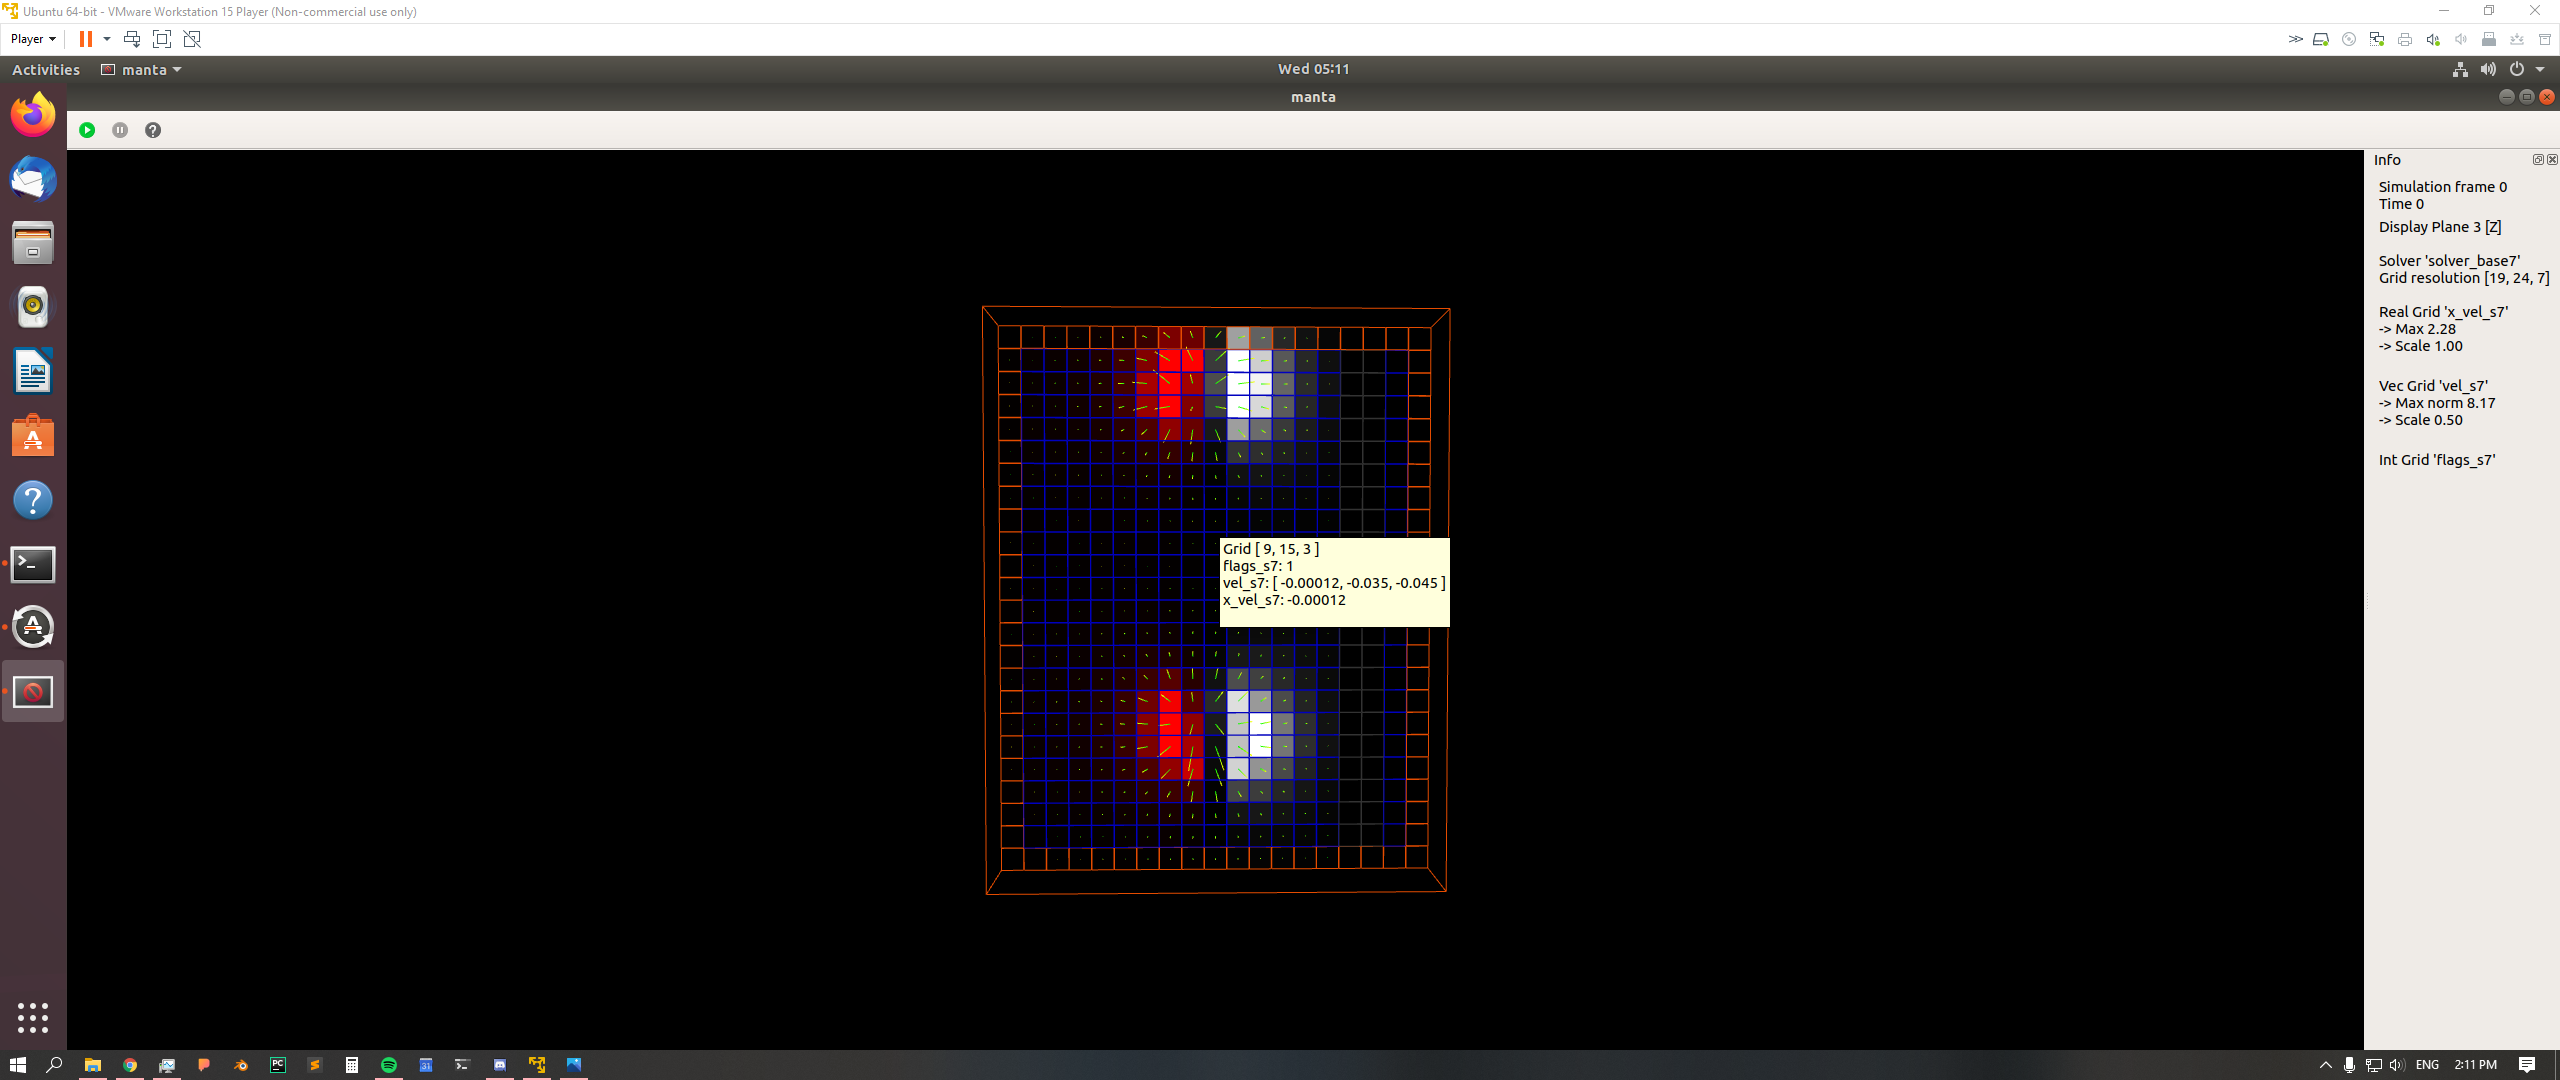
\includegraphics[scale = 0.165]{mgui_2.png}
		\caption{Prędkość cząstek.}
	\end{figure}
	
	\pagebreak
	
	\vspace{12mm}
	\section{Wnioski}
	Z naszych symulacji można wyciągnąć następujące wnioski:
	
	\subsection{Co doświadczalnie na podstawie uzyskanych wyliczeń i obrazów uzyskaliśmy~i potwierdziliśmy}
	\begin{itemize}
		\item Im większa temperatura dymu, rozprzestrzenia się on szybciej.
		\item Im cieplejszy dym, tym unosi się on wyżej, przez co czas wietrzenia jest dłuższy - w naszym modelu przy temperaturach w stosunku 1:16, czas wywietrzania wynosił 1.5 raza dłużej
		\item Czas wywietrzania jest zależny od sumarycznej mocy oraz rozmieszczenia wentylatorów
		\item Zatrzymanie źródła dymu nie niweluje zagrożenia w całości, gdyż w sali on się nadal utrzymuje
		\item Im większa temperatura dymu, tym mniejsza jego gęstość
	\end{itemize}
	
	\subsection{Z jakimi głównymi problemami się zmagaliśmy}    
	\begin{itemize}   
		\item Bardzo ciężko stworzyć wirtualny model idealnie odwzorowujący rzeczywiste sytuacje
		\item Symulacje są bardzo kosztowne obliczeniowo
	\end{itemize}
	
	\vspace{12mm}
	\section{Podsumowanie}
	Nasze przykładowe symulacje jedynie cząstkowo obejmują całą złożoność problemu rozprzestrzeniania się dymu, jednak stworzony przez nas uniwersalny system modelowania rozchodzenia się dymu jest pełen możliwości - lecz nie jest to jeszcze projekt kompletny i zamknięty. 
	
	\medskip
	\medskip
	\noindent Ciekawym kierunkiem rozwoju naszego projektu byłoby dodanie różnorodnych skryptów pozwalających na obliczanie oraz prezentowanie statystyk m.in zakresu widoczności w funkcji odległości przy różnym poziomie zadymienia pomieszczenia, wartości średniej temperatury powietrza w zależności od wysokości jej pomiarów. 
	
	\medskip
	\medskip
	\noindent Przede wszystkim należy jednak rozważyć zadania, jakie miałby realizować program. Wymagania wobec symulatora CFD będą różnić się w zależności, czy badamy rozwój pożaru w budynku, czy tworzymy animację dymu na potrzeby grafiki komputerowej. W jednym przypadku priorytetem może być wierność fizyce, a w drugim wizualna atrakcyjność.
	
	\newpage
	
	\begin{thebibliography}{}
		\bibitem{pa} Wikipedia [online] [dostęp: 08.04.2020]. Dostępny w Internecie, link:
		\href{https://pl.wikipedia.org/wiki/Dyspersja_(chemia_fizyczna)}{"układ dyspersyjny Wikipedia"}
		\bibitem{pa} Encyklopedia PWN [online] [dostęp: 08.04.2020]. Dostępny w Internecie, link: \href{https://encyklopedia.pwn.pl/haslo/dym;3895349.html}{"dym definicja PWN"}
		\bibitem{pa} Ronald Fedkiw, Jos Stamy, Henrik Wann Jensen: \emph{Visual Simulation of Smoke}
		\bibitem{pa} Nick Foster and Dimitris Metaxas: \emph{Modeling the Motion of a Hot, Turbulent Gas}
		\bibitem{pa} Eren Algan: \emph{REAL-TIME SMOKE SIMULATION}
		\bibitem{pa} Marinus Rorbech: \emph{REAL-TIME SIMULATION OF SMOKE USING GRAPHICS HARDWARE}
		\bibitem{pa}Ryszard Gryboś: \emph{Podstawy mechaniki płynów. Część 1}
		\bibitem{pa}Lorena A. Barba, Gilbert F. Forsyth: \emph{12 steps to Navier-Stokes}
		\bibitem{pa}Jos Stam: \emph{Stable Fluids}
		\bibitem{pa}David Potter: \emph{ Metody obliczeniowe fizyki}
		\bibitem{pa}David Cline, David Cardon, Parris K. Egbert: \emph{Fluid Flow for the Rest of Us: Tutorial of the Marker and Cell Method in Computer Graphics}
		\bibitem{pa}\href{https://pypi.org/project/pyjet/}{https://pypi.org/project/pyjet/}
		\bibitem{pa}\href{https://numpy.org/}{https://numpy.org/}
		\bibitem{pa}\href{https://fluidityproject.github.io/}{https://fluidityproject.github.io/} \bibitem{pa}\href{https://fluidenginedevelopment.org/pdoc/}{https://fluidenginedevelopment.org/pdoc/}
		\bibitem{pa}\href{http://mantaflow.com/}{http://mantaflow.com/}
		\bibitem{pa}\href{http://mantaflow.com/gui.html}{http://mantaflow.com/gui.html}
		\bibitem{pa}\href{https://www.blender.org/}{https://www.blender.org/}
		\bibitem{pa}\href{https://docs.blender.org/manual/en/latest/}{https://docs.blender.org/manual/en/latest/}
		\bibitem{pa}\href{https://www.nvidia.com/pl-pl/}{https://www.nvidia.com/pl-pl/}
		\bibitem{pa}KRYSTYNA JEŻOWIECKA-KABSCH, HENRYK SZEWCZYK: \emph{MECHANIKA PŁYNÓW }
		
		
	\end{thebibliography}
	
\end{document}